\documentclass[]{article}
\usepackage[margin=2.5cm]{geometry}
\usepackage{graphicx}

%opening
\title{Grundlagen der Startplanung}
\author{Ida Hönigmann}

\newenvironment{question}{\vspace{8mm}\noindent\bfseries}{\\}

\begin{document}

\maketitle

\section{Einführung in das Semesterprogramm}
\begin{question}
	Erläutern Sie wesentliche Faktoren, die die Entwicklung der Stadt beeinflussen. Gruppieren Sie diese.
\end{question}
wirtschaftlich, sozial, demografisch, kulturell, umweltbezogen, rechtlich, technisch

\begin{question}
	''Stadtplanung ist eine Wissenschaft, eine Kunst, eine politische Bestrebung.'' Diskutieren Sie dies.
\end{question}
\begin{itemize}
	\item Wissenschaft: Kenntnisse der Stadtstruktur, Dienstleistungen und Beziehung der Bestandteile und Verkehrsbewegungen zu gewinnen;
	\item Kunst: Ziel der Bestimmung der Bodenordnung, Anordnung von Flächennutzungen und Verkehrswegen und Gebäudeentwurfes nach Grundsätzen, die Ordnung, Gesundheit und Wirtschaftlichkeit sichern;
	\item politische Bestrebung: um Grundsätzen Wirksamkeit zu verliehen.
\end{itemize}

\begin{question}
	Was verstehen Sie unter ''Ordnungsaufgaben'', was unter ''Gestaltungsaufgaben'' in der Stadtplanung?
\end{question}
\begin{itemize}
	\item Ordnungsaufgaben: Fragen des Flächenanspruchs und der wechselseitigen Zuordnung verschiedener Nutzungen
	\item Gestaltungsaufgaben: dreidimensionale Gestaltung des städtischen Raumes
\end{itemize}

\section{Wien - Geschichte, Gegenwart, Zukunftsperspektiven}
\begin{question}
	Erläutern Sie die zentralen Rahmen- und Ausgangsbedingungen zum STEP 2025 in Wien. Wie reagiert der STEP auf diese Herausforderungen?
\end{question}
Ausgangsbedingungen: Wachstum an Einwohnerzahlen prognostiziert, Zunehmende Verflechtung mit Umgebender Metropolregion, Klimaänderungen deutlicher merkbar

Herausforderungen siehe Frage weiter unten

\begin{question}
	Benennen Sie einige zentrale Phasen der Wiener Stadtentwicklung und richten Sie den Fokus dabei vor allem auf die Entwicklung ab Mitte des 19. Jahrhunderts!
\end{question}
Wien entwickelte sich auf dem Ort eines römischen Legionslagers zu einer immer bevölkerungsreicheren Stadt. Aus Verteidigungszwecken wurde ein Befestigungswall um die Stadt errichtet, was jedoch ab dem 19. Jahrhundert zu einem Platzmangel führt. Eines der entscheidenden Projekte für die Stadt Wien ist daher der Umbau der Verteidigungsmauern zur Ringstraße.

Ein weiteres großes Projekt war die Regulierung der Donau. Vor und im 19. Jahrhundert kam es immer wieder zu Überschwemmungen, weswegen immer mehr Arme der Donau abgesperrt wurden. Nach dem Hochwasser im Jahr 1954 war klar, dass zusätzlich ein Entlastungsgerinne notwendig war. Der Bau dieses Neuen Donau ließ die sogenannte Donauinsel entstehen.

Im Zuge von Stadterweiterungen wird Anfang des 20. Jahrhunderts ist immer wieder vom kreisförmigen Stadtbild und dem grünen Ring um Wien die rede.

Viele Wiener lebten um 1900 in schlechten Wohnbedingungen. Um die Wohnungsnot zu bekämpfen werden in der Zeit des roten Wiens Wohnungsbauten von der Gemeinde Wien gebaut. Diese Wohnungen entsprechen wesentlich besseren Standards als davor in Wien üblich. Es wird begonnen Richtlinien und Bestimmungen in Form von Bauordnungen zu verordnen.

Nach dem zweiten Weltkrieg entstanden durch den steigenden Mobilisierungsgrad ermöglicht viele Entwicklungen an den Rändern der Stadt Wien. Es wurde Auto-freundlich gebaut und umgebaut. Allerdings wurde diese Entwicklung auch kritisch gesehen. So wird der Fokus der Stadtentwicklung in Wien auf die Erhaltung und Erneuerung gelegt.

Nach dem Fall der eisernen Mauer rückt Wien weiter ins Zentrum Europas. Es kommt immer wieder Überlegungen über eine Kooperation mit Bratislava.

\begin{question}
	Worin begründen sich die besonderen Herausforderungen der Wiener Stadtentwicklung?
\end{question}
Herausforderung: Strategien und Instrumente der Stadtentwicklung weiterzuentwickeln sodass Qualitätsstandards erhalten und neue, zukunftsgerichtete Qualitäten ermöglichen;

\begin{itemize}
	\item standortwirtschaftliche und infrastrukturelle Rahmenbedingungen für Investor*innen und Entwickler*innen sodass rasch, elastisch und innovativ auf Veränderungen reagiert werden kann und den Interessen und Bedürfnissen der Bevölkerung entsprochen wird;
	\item gebaute, (frei-)räumliche und ökologische Substanz der Stadt fit zu machen für Wachstum, Erhalten, Erneuern, Transformieren.;
	\item stabiles soziales Gleichgewicht; Diversität und Gleichstellung;
	\item kollektive Verantwortung und Kooperationsaufgabe von Politik, Wirtschaft und Bevölkerung;
	\item Prozesse von Planung, Managements, Umsetzung partizipativ und effizient gestalten.
\end{itemize}

\begin{question}
	Erläutern Sie wesentliche im STEP 2025 dokumentierte Prinzipien der Wiener Stadtentwicklung!
\end{question}
Aufbruch durch Wachstum und Entwicklungsdynamik kommt der ganzen Stadt zugute. lebenswerte Stadt bleiben (leben, arbeiten, lernen, austauschen). attraktives Wien für alle erlebbar sein.
Wettbewerbsfähigkeit und Unternehmergeist, Leistbarkeit, soziale Gerechtigkeit, Integration, ressourcenschonende Klima- und Umweltschutzpolitik alles gleich gewichtet.

STEP berücksichtigt Besonderheiten, Stärken und Schwächen des Standorts Wien.
STEP bezieht Fachkonzepten mit ein.
STEP ist für die Wiener Stadtentwicklung handlungsleitend.

\begin{question}
	Erläutern Sie die wesentlichen Ziele der vier Handlungsbereiche des STEP 2025!
\end{question}
\begin{itemize}
	\item Wir leisten uns Stadt
	
	\item Wien baut auf
	
	Qualitätsvolle Stadtstruktur und vielfältige Urbanität
	
	\item Wien wächst über sich hinaus
	
	Wachstum und Wissensgesellschaft transformieren die Metropolregion
	
	\item Wien ist vernetzt
	
	Weitsichtig, robust und tragfähig für Generationen
\end{itemize}

\begin{question}
	Diskutieren Sie den im STEP 2025 zum Ausdruck gebrachten Anspruch ''Wir leisten uns Stadt!'' (S. 12ff)
\end{question}

\begin{itemize}
	\item Entwicklung, Nutzung und Optimierung öffentlich-rechtlicher Instrumente zur Bodenmobilisierung
	\item Etablieren von Methoden zur Einbeziehung von Privaten in die Realisierung von Infrastrukturen
	\item Öffentlich und Privat als Partner in der Stadtentwicklung
	\item Zielgebiete für die Stadtentwicklung nutzen
	\item Kooperation mit Bezirken und in der Region
	\item Beteiligung professionalisieren und verstetigen
\end{itemize}

gesellschaftliche Integration, hohe urbane Qualität, soziales Gleichgewicht

intensiver wirtschaftlicher Wettbewerb, dynamisches Bevölkerungswachstum, hoher Investitionsbedarf, knappe Ressourcen

intelligent ressourcenschonend, sozial ausgleichend, geschlechtergerecht, wirtschaftlich wettbewerbsstärkend

\begin{question}
	Diskutieren Sie den Anspruch des STEP 2025 an eine qualitätsvolle Stadtstruktur und vielfältige Urbanität! Benennen Sie die zentralen Ziele! (S. 34)
\end{question}

\begin{itemize}
	\item Innenwachstum vor Außenwachstum
	\item Wohnraumentwicklung im bereits bebauten Stadtgebiet und mehr Qualität in bestehenden Strukturen
	\item Stärkung der polyzentralen Stadtstruktur
	\item Wachstum entlang vorhandener Infrastrukturen
	\item Kompakte Bauformen halten Siedlungswachstum in Grenzen
	\item Attraktives Grün- und Freiflächenangebot ermöglicht qualitätsvolle Urbanität
	\item Städtebau für eine smarte Stadt der Ressourcenschonung und der kurzen Wege
\end{itemize}

Ziele: Stadt der kurzen Wege, bis 2025 Platz für 120.000 Wohnungen, Ungenutzte Flächen im inneren der Stadt umbauen und integrieren, Plusenergiehaus

\begin{question}
	Was sind die im STEP 2025 dokumentierten Aspekte der Flächensicherung für das Stadtwachstum? (S. 48ff)
\end{question}
bereits bestehende Brachflächen und nicht mehr genutzte Bahnhofsareale, Flächen in Außenbezirken und am Stadtrand, insgesamt ergibt das Flächen für 135.000 Wohneinheiten und mehreren Millionen Quadratmeter Büro- und Zentrumsnutzung

\begin{itemize}
	\item Flächenaktivierung
	\item Qualitätsvolle Urbanität
	\item Wohnfolgeeinrichtungen
	\item Langfristige Siedlungserweiterung
	\item Öffentlicher Raum und Stadtentwicklung
	\item Weiterentwicklung des Energiesystems
	\item Städtebau in der Smart City
\end{itemize}

\begin{question}
	Was versteht der STEP 2025 unter einer ''ausgewogenen, polyzertrischen Standortentwicklung''? (S. 64)
\end{question}
Stadt der kurzen Wege; kleinteilige Verteilung von Zentren; Stärkung etablierter Zentren; gezielte Entwicklung neuer Zentren; vor allem in Flächenbezirken mit hohem Bevölkerungswachstum

\begin{question}
	Diskutieren Sie das Leitbild zur Siedlungsentwicklung! (S. 67)
\end{question}
Siehe Grafik \ref{fig:leitbildsiedlungsentwicklung}

\begin{figure}
	\centering
	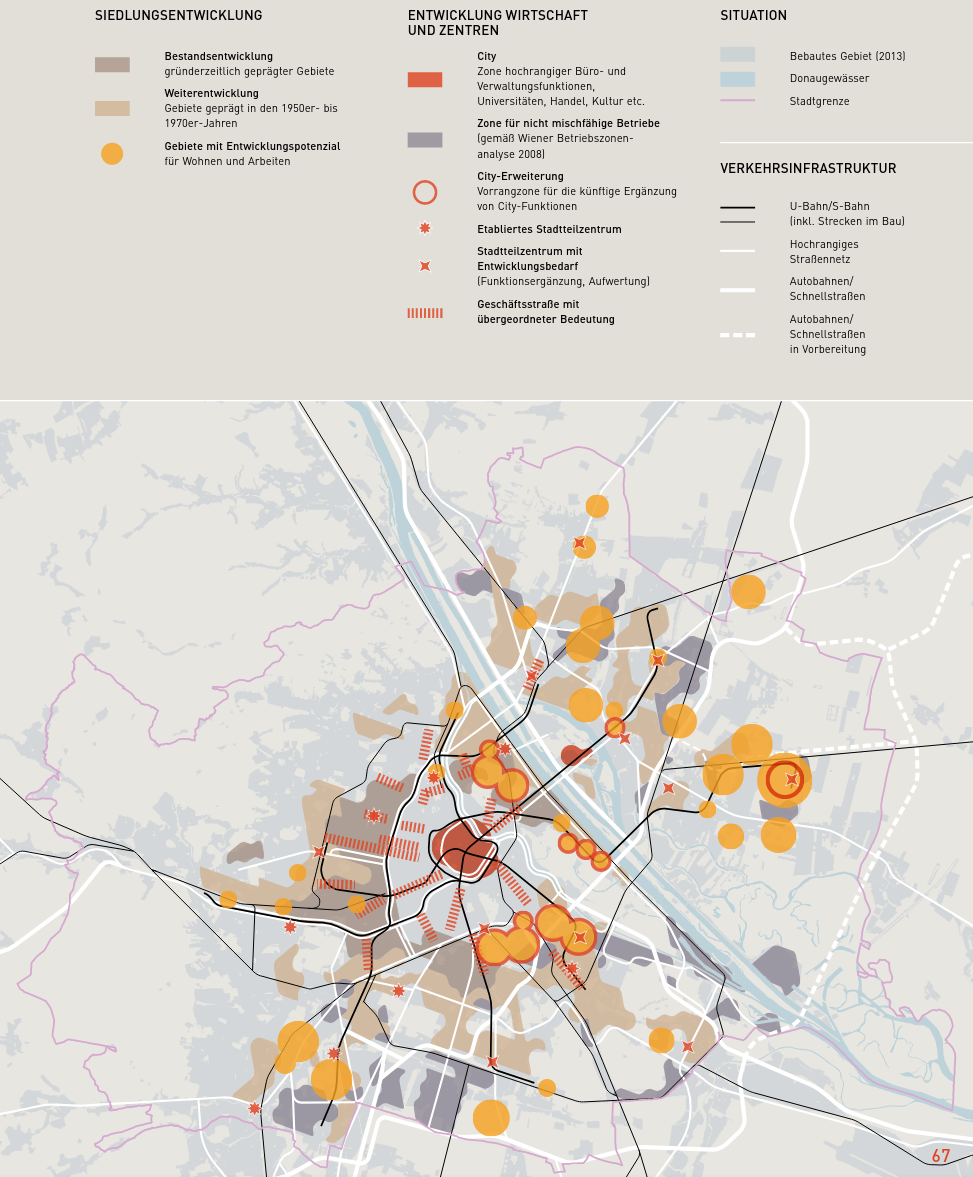
\includegraphics[width=0.9\linewidth]{images/leitbild_siedlungsentwicklung}
	\caption{Leitbild Siedlungsentwicklung}
	\label{fig:leitbildsiedlungsentwicklung}
\end{figure}


\begin{question}
	Diskutieren Sie den Anspruch and die Entwicklung der Metropolregion! (S. 88ff)
\end{question}
Starke Vernetzung mit Umland; Grenzen verschwimmen; durch kurze Wege von etwa St. Pölten, Wiener Neustadt, Tulln nach Wien und umgekehrt viele Pendlerbewegungen; Industrie siedelt sich auch in umgebenden Gemeinden an

Nachhaltige Kooperation, Stadtregionale Governance-Strukturen, Ressourcen sichern und bündeln

\begin{question}
	Was sind Fachkonzepte zum STEP25?
\end{question}
Begleitende Dokumente zum STEP die spezifische Information und Herausforderungen und Lösungsansätze zu verschiedensten Spezialgebieten der Stadtentwicklung enthalten. z.B. Produktive Stadt, Mittelpunkt des Städtischen Lebens, Grün- und Freiraum, Öffentlicher Raum, Mobilität, Hochhäuser, Partizipative Stadtentwicklung, Masterplan Gründerzeit

\begin{question}
	Welche Wirkungen entfalten STEP 2025 und die Fachkonzepte zum STEP?
\end{question}
TODO

\begin{question}
	Welchen Stellenwert besitzt die Smart City Rahmenstrategie der Stadt Wien?
\end{question}
langfristige Dachstrategie, Zielhorizont 2050

\begin{question}
	Erläutern Sie die drei Handlungsfelder auf die sich die Smart City Rahmenstrategie der Stadt Wien bezieht!
\end{question}
\begin{itemize}
	\item Ressourcen (Energie, Mobilität, Infrastruktur, Gebäude)
	\item Lebensqualität (Soziale Inklusion, Partizipation, Gesundheit, Umwelt)
	\item Innovation (Bildung, Wirtschaft, Forschung, Technologie)
\end{itemize}

\section{Theorie und Methodik der Stadtplanung}
\begin{question}
	Erläutern Sie die wesentlichen Grundfunktionen der räumlichen Planung!
\end{question}

\begin{itemize}
	\item Vernetzung unterschiedlicher Interessen
	\item Zukunftsperspektive
	\item Abbau von Konflikten zwischen Raumansprüchen
	\item Verteilung der Nutzungen und Gestaltung der Raumansprüche
	\item Verhindern vermeidbarer Unterschiede der Lebensbedingungen
	\item Erhaltung natürliche und kulturelle Elemente
	\item Schonung naturgebundener Ressourcen
\end{itemize}


\begin{question}
	Woran orientiert sich die Planung? Stellen Sie das Wirkgeflecht grafisch dar!
\end{question}

\begin{itemize}
	\item Rechtsvorgaben
	\item politische Zielsetzungen
	\item politische Programme und Richtlinien
	\item Erkenntnisse aus Wissenschaft und Praxis
	\item Referenzprojekte und historische Vorbilder
	\item Zielsetzungen und Qualitätsansprüche aus Bevölkerung
	\item eigene Erfahrungen, Werthaltungen und Prinzipien
\end{itemize}

insgesamt eine Mischung aus

\begin{itemize}
	\item allgemein und speziell,
	\item verbindlich und unverbindlich,
	\item normativ und deskriptiv,
	\item kurzfristig und langfristig
	\item Vorschriften, Zielsetzungen, Wertsetzungen und Handlungsprinzipien
\end{itemize}

\begin{figure}[h!]
	\centering
	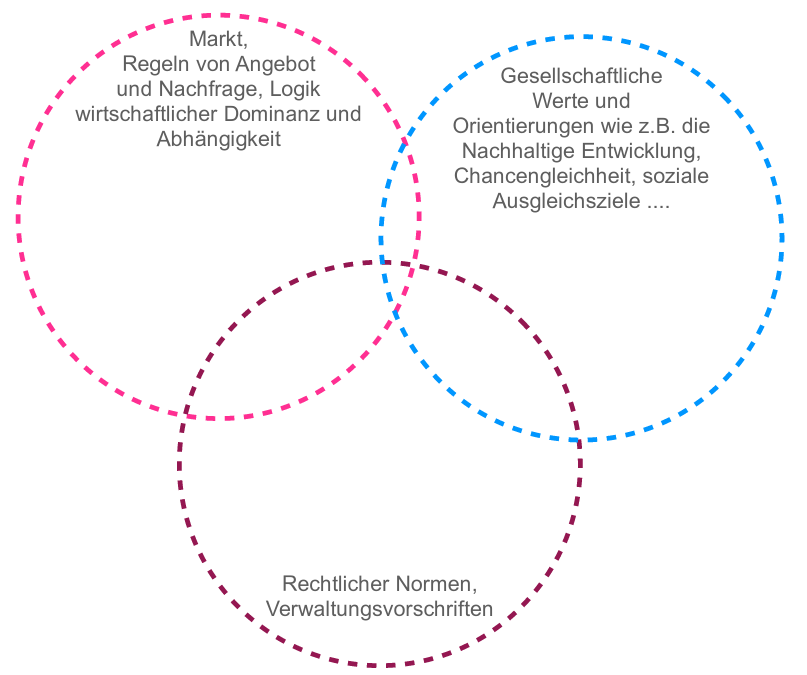
\includegraphics[width=0.5\linewidth]{images/planung_wirkgeflecht}
	\label{fig:planungwirkgeflecht}
\end{figure}


\begin{question}
	Diskutieren Sie das Verhältnis von Planung, Politik und Verwaltung!
\end{question}
\begin{itemize}
	\item Planung: Entscheidungsvorbereitung
	\item Politik: Entscheidung über Alternativen
	\item Verwaltung: Administrativer Vollzug
\end{itemize}

In Praxis: Vermischung der Ebenen z.B. bereits Auswahl von nur wenigen Alternativen in Planungsphase oder Politik gibt Rahmenbedingungen zur Planung vor.


\begin{question}
	Wer entwickelt die Stadt? Welche Aufgabe nimmt die Stadtplanung in dem Akteursgeflecht ein?
\end{question}
\begin{itemize}
	\item Planungsträger - Auftraggeber der Planung z.B. Gemeinde
	\item Planer - Bearbeitung der Pläne unter fachlichen Aspekten z.B. Stadtplanungsamt
	\item Entscheider - Entscheiden über Entwürfe z.B. Gemeinderat
	\item Durchführender - Durchführen von Maßnahmen z.B. Bauträger
	\item Beteiligte/Betroffene - Personen und Institutionen die von den Maßnahmen berührt werden z.B. Anwohner, Investoren
\end{itemize}


\begin{question}
	Was müssen Pläne leisten? Welche Anforderungen sind mit dem Plan verknüpft?
\end{question}
\begin{itemize}
	\item Orientierung, Rechtssicherheit
	\item Inhalte bildlich vermitteln, Argumentationen abbilden, Dialoge anregen
\end{itemize}

Anforderungen:
\begin{itemize}
	\item Vermittlung / Kommunikation
	\item Steuerungsintention
	\item Überschaubare und kontrollierbare Ziel-Mittel-Verknüpfung
	\item Festlegung von Prioritäten und Präferenzen
	\item Zeitlich festgelegte Verwirklichungsstufen
	\item Grafische Darstellung
\end{itemize}


\begin{question}
	In der Planungspraxis wird zwischen einer langfristig orientierten Querschnittplanung und einer projekt- bzw. aufgabenspezifischen Planung unterschieden. Erläutern Sie dies.
\end{question}
\begin{itemize}
	\item Langfristig orientierte Querschnittsplanung:
	
	z.B. Stadtentwicklungskonzept
	
	\begin{itemize}
		\item Darstellung von Zielen, Prioritäten, Alternativen, Perspektiven
		\item langfristige Orientierung
		\item Stadt- bzw. Gemeindegebiet
		\item Maßstab: 1:25.000 bis 1:10.000
		\item Schwerpunktsetzend
		\item flexibel/variabel
		\item präventiv/perspektivisch
		\item informell
	\end{itemize}

	\item Projekt- bzw. Aufgabenbezogene Planung:
	
	z.B. Gestaltungsentwurf
	
	\begin{itemize}
		\item Auf kurzfristige Umsetzung angelegt
		\item Maßstab: 1:500 bis 1:200
		\item Präzise
		\item Umsetzungsbezogen
	\end{itemize}
\end{itemize}


\begin{question}
	Erläutern Sie wesentliche Herausforderungen der Innenstadtentwicklung!
\end{question}
Beschränkter Platz, Verkehr, Mobilität, Aufenthaltsqualität, Erlebnisfaktor, Wohnorte, Gewerbebetriebe, Emissionen


\begin{question}
	Auf welchen Steuerungsformen basiert die Raumplanung?
\end{question}
\begin{itemize}
	\item Ordnungsinstrumente: Raumpläne, Ge- und Verbote, planerische Stellungnahmen
	\item Marktliche Instrumente: Zielvereinbarungen, steuerliche Anreize, Vertragslösungen
	\item Diskursive Instrumente: Masterpläne, Entwicklungskonzepte
\end{itemize}


\begin{question}
	Diskutieren Sie wesentliche Unterscheidungsmerkmale zwischen der Objektplanung und der Stadtplanung / örtlichen Raumplanung!
\end{question}
siehe Grafik \ref{fig:vergleichstaedtebauobjektplanung}
\begin{figure}[h!]
	\centering
	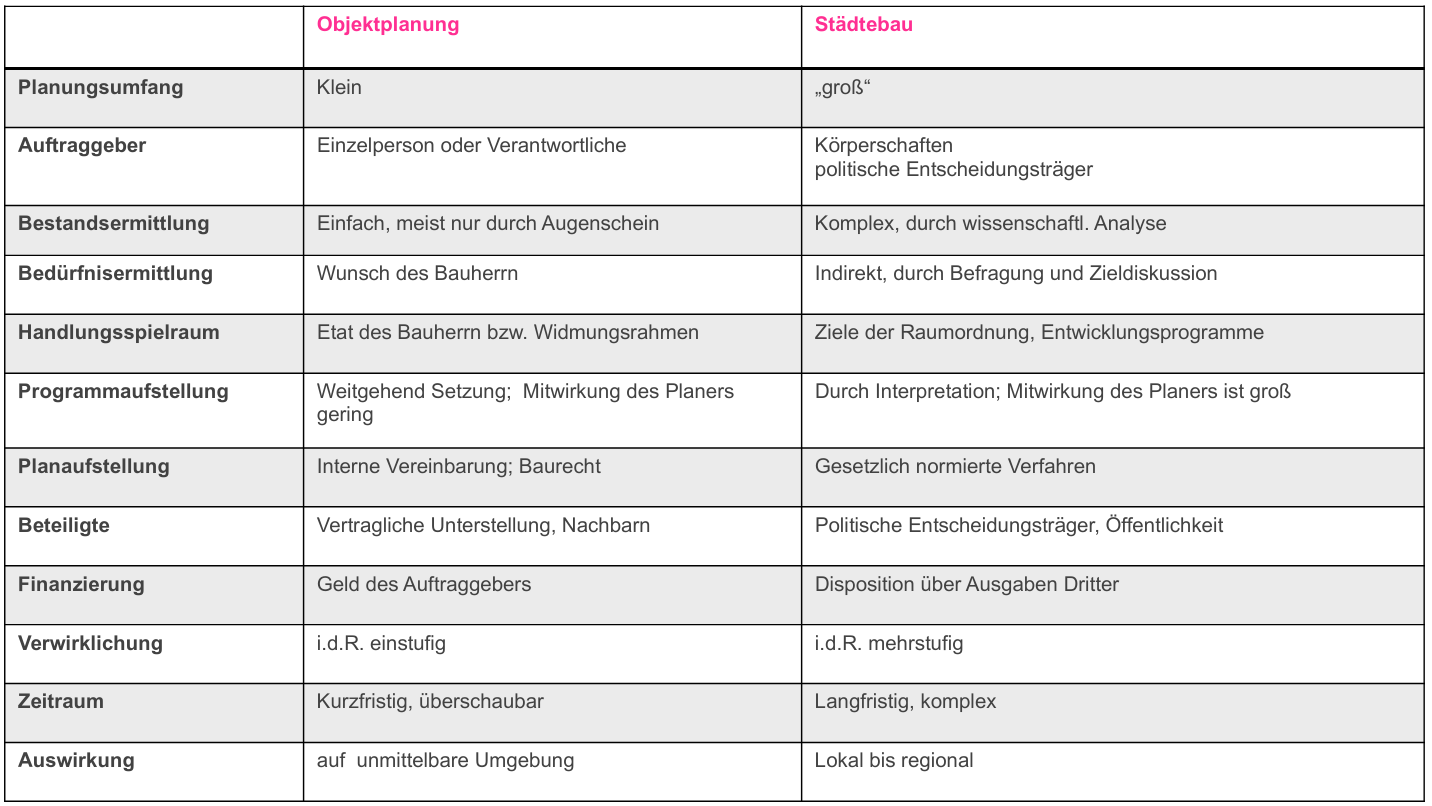
\includegraphics[width=0.7\linewidth]{images/vergleich_staedtebau_objektplanung}
	\caption{Tabellarischer Vergleich}
	\label{fig:vergleichstaedtebauobjektplanung}
\end{figure}


\begin{question}
	Jeder Entwurfsprozess folgt einer wissenschaftlichen Methodik. Nehmen Sie dazu Stellung und stellen Sie die Entwurfsmethodik in den einzelnen Schritten dar (Diagramm, Erläuterungen)!
\end{question}
\begin{enumerate}
	\item Erfassen und Analysieren
	\item Klärung der Wertmaßstäbe und Zielvorgaben
	\item Abgrenzung des planerischen Handlungsspielraumes
	\item Abwägung der Alternativen
	\item Umsetzung der getroffenen Entscheidung
	\item Verwirklichung des Planes
\end{enumerate}


\begin{question}
	Welche Informationsebenen umfasst die Bestandsanalyse?
\end{question}
\begin{itemize}
	\item Räumliche Information: z.B. Bebauung, Freiflächen, Infrastruktur
	\item Handlungsinformation: z.B. Planungsrecht, Planungs- und Investitionsabsichten
	\item Soziale Information: z.B. sozio-ökonomische Entwicklung, soziale Schichten, Bedarfsanalyse, Eigentumsverhältnisse
\end{itemize}


\begin{question}
	Benennen Sie einige Techniken der Bestandsaufnahme in der Stadtplanung!
\end{question}
TODO


\section{Instrumente der Örtlichen Raumplanung}
\begin{question}
	Was ist unter dem Begriff ''ÖROK'' zu verstehen? Welche Aufgaben kommen der ÖROK zu?
\end{question}
Österreichische Raumordnungskonferenz ist freiwilliges, gemeinsames Übereinkommen von Bund, Ländern, Städten und Gemeinden.

wurde zur besseren Abstimmung als politisches Organ gegründet.

besteht aus Mitgliedern der Bundesregierung, den Landeshauptleuten, den Präsidenten von Städte- und Gemeindebund und Wirtschafts- und Sozialpartner (in beratender Funktion)

wichtigste Aufgabe: Erstellung des ÖREK (Österreichischen Raumentwicklungskonzeptes) alle zehn Jahre



\begin{question}
	Welche Kompetenzen in raumplanerischen Fragen hat die ÖROK?
\end{question}
Erstellung des ÖREK als gemeinsame, gesamtstaatliche Strategie zur Raumplanung

Grundlagenprojekte wie Raumordnungsbericht, ÖROK-Atlas, Prognosen, ÖROK-Schriftenreihe

National Contact Point für fragen der Raumplanung


\begin{question}
	Erläutern Sie wichtige Zielsetzungen und Ansprüche des ÖREK 2030!
\end{question}
\begin{itemize}
	\item Klimaschutz, Energiewende
	\item Kompakte Siedlungsstrukturen
	\item gleichwertige Lebensbedingungen
	\item polyzentrische Strukturen
	\item Leistungsfähige Achsen und Knoten des öffentlichen Verkehrs
	\item regional und funktionale Lebensräume, lokale und regionale Stärken
	\item Resilienz
	\item Kulturlandschaft
\end{itemize}


\begin{question}
	Im ÖREK 2030 sind einige Megatrends benannt. Welche sind dies?
\end{question}
\begin{itemize}
	\item Klimawandel und Klimakrise
	\item Digitalisierung
	\item Globalisierung
	\item Demographischer Wandel
	\item Gesellschaftlicher Wandel
	\item Wissensgesellschaft
	\item Urbanisierung und Suburbanisierung
	\item Steigender Energiebedarf
\end{itemize}


\begin{question}
	Was verbirgt sich in dem 10-Punkte-Programm des ÖREK 2030?
\end{question}
\begin{enumerate}
	\item Raumentwicklung auf Klimaneutralität und Energiewende fokussieren
	\item Flächeninanspruchnahme und Bodenversiegelung reduzieren
	\item Orts- und Stadtkerne stärken sowie Raum für Baukultur eröffnen
	\item Freiräume ressourcenschonend und für den Klimaschutz gestalten
	\item Erreichbarkeit sichern und klimaneutral gestalten
	\item Klimawandelanpassung durch Raumentwicklung und Raumordnung unterstützen
	\item Daseinsvorsorge für gleichwertige Lebensbedingungen gestalten und leistbares Wohnen sichern
	\item Regionale Wertschöpfungsketten und Kreislaufwirtschaft stärken
	\item Die Digitalisierung nutzen und regionale Innovationssysteme stärken
	\item Government und Governance als Querschnittsthema integrieren
\end{enumerate}


\begin{question}
	Welche Raumtypen werden im ÖREK 2030 definiert?
\end{question}
\begin{itemize}
	\item Stadtregionen der Landeshauptstädte
	\item Stadtregionen und ländliche Verdichtungsräume
	\item Achsenräume entlang hochrangiger Verkehrsinfrastruktur
	\item Ländliche Tourismusregionen
	\item Ländlicher Raum mit geringer Bevölkerungsdichte
\end{itemize}


\begin{question}
	Benennen Sie einige exemplarische Herausforderungen in den einzelnen Raumtypen!
\end{question}
\begin{itemize}
	\item Schutz und Sicherheit
	\item Leben an mehreren Orten
	\item Baulandmobilisierung
	\item Leerstände
	\item ausgewogene Stadt- und Regionalentwicklung
	\item Produktion
	\item Digitalisierung
	\item Mobilitätsangebote
\end{itemize}


\section{Instrumente der Stadtplanung}
\begin{question}
	Erläutern Sie die unterschiedlichen Typen von Plänen (nach Albers)!
\end{question}
siehe Grafik \ref{fig:typenvonplaenen}

\begin{figure}
	\centering
	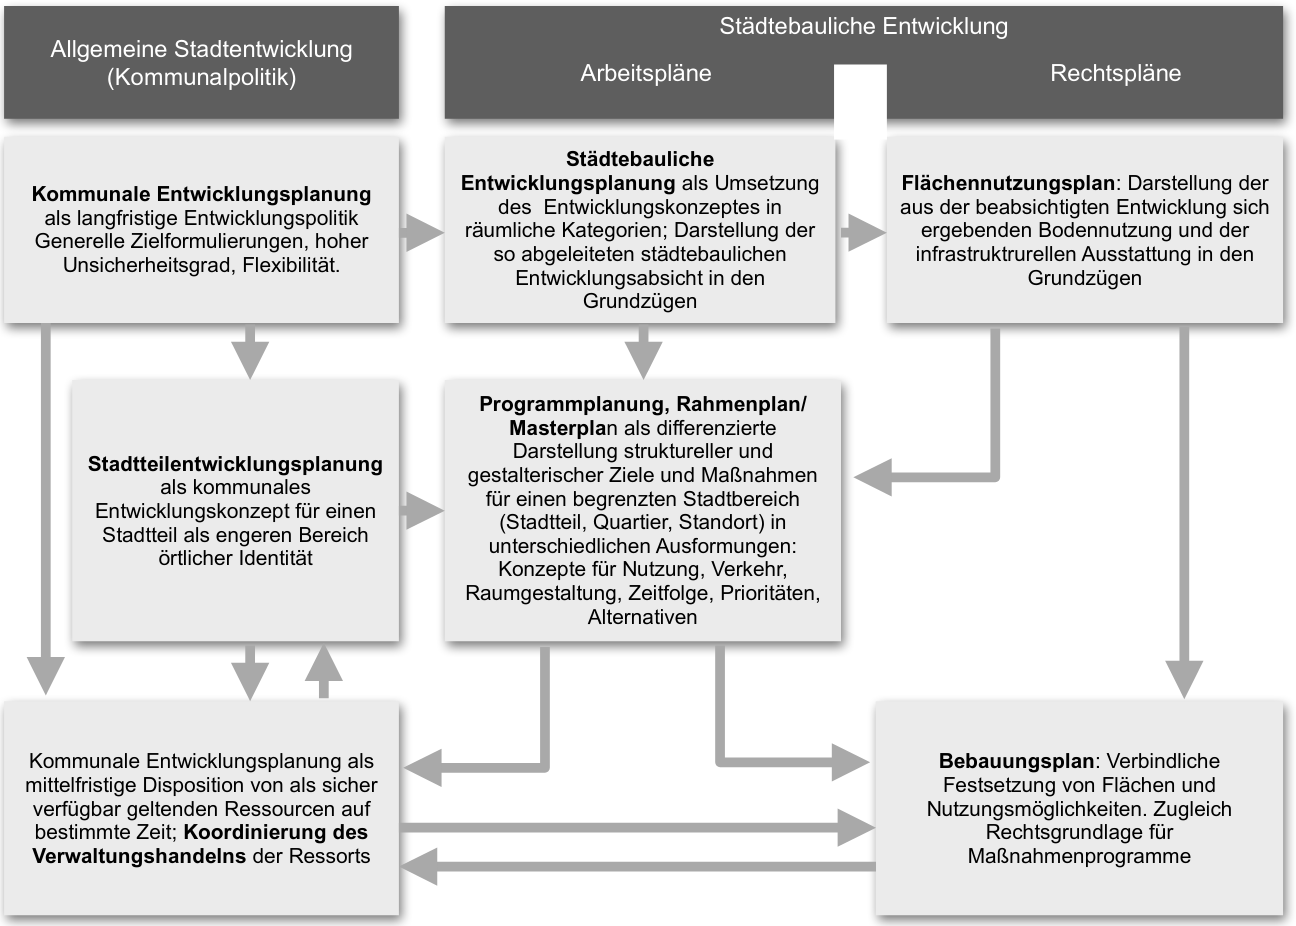
\includegraphics[width=0.7\linewidth]{images/typen_von_plaenen}
	\caption{Type von Plänen nach Albers}
	\label{fig:typenvonplaenen}
\end{figure}



\begin{question}
	Erläutern Sie die Unterschiede zwischen formellen und informellen Instrumente! Benennen Sie Beispiele!
\end{question}

\begin{itemize}
	\item Formell: hierarchisch, gesetzlich normiert, Rechtsverbindlich
	
	z.B. Flächenwidmungsplan, Bebauungsplan
	
	\item Informell: Fachübergreifend, Flexibel, gesetzlich nicht normiert, nicht hierarchisch, Dialogorientiert
	
	z.B. Leitbildprozess, Zukunftskonferenz, Städtenetz
\end{itemize}


\begin{question}
	Erläutern Sie die wesentlichen Instrumente der Raumplanung auf der örtlichen Ebene!
\end{question}
\begin{itemize}
	\item Sektoralpolitiken, Föderprogramme, Leitlinien
	\item Koordination von Empfehlungen, Ressortplanung
	\item Gesetzgebung, Fachplanung, Landesentwicklungsprogramm, Regionales Raumordnungsprogramm, Sektorales Raumordnungsprogramm
	\item Baubewilligungen, Örtliches Entwicklungskonzept, Flächenwidmunsplan, Bebauungsplan
\end{itemize}


\begin{question}
	Ordnen Sie Plandarstellungen den Instrumenten zu!
\end{question}
\begin{itemize}
	\item Landesentwicklungsprogramm: enthält Ziele und Maßnahmen für gesamtes Landesgebiet
	\item Regionales Raumordnungsprogramm: enthält wichtige Vorgaben für örtliche Raumplanung für Teilbereiche des Landes
	\item Örtliche Entwicklungskonzept: enthält grundsätzliche Ziele, Maßnahmen und Finanzierung zu langfristigen, strategischen Entwicklungen in der Gemeinde
	\item Flächenwidmungsplan: enthält parzellenschafte Festlegung der Bodennutzung des gesamten Gemeindegebiets
	\item Bebauungsplan: enthält Maße und Gestaltungsregeln für die Bebauung innerhalb von Parzellen
\end{itemize}


\section{Instrumente auf der Örtlichen Ebene}
\begin{question}
	Was verstehen Sie unter einem Örtlichen Raumordungsprogramm in NÖ? Was sind seine Bestandteile?
\end{question}
Rechtlicher Rahmen für Raumplanung in NÖ

beschäftigt sich mit langfristigen (5 - 10 Jahre) Zielen von Gemeinden und notwendigen Maßnahmen

Bestandteile: Örtliches Entwicklungskonzept, Flächenwidmungsplan

\begin{question}
	Erläutern Sie grundlegende Ansprüche an das Örtliche Entwicklungskonzept!
\end{question}
\begin{itemize}
	\item Zeitlicher Aspekt: Langfristig und Kontinuität
	\item Gesellschaftlicher Aspekt: Interessenabwägung und Interessensausgleich
	\item Rechtlicher Aspekt: Rechtssicherheit und Nachvollziehbarkeit
	\item Ökologischer Aspekt: Vorsorge und Nachhaltigkeit
	\item Funktionaler Aspekt: Trennung und Bündelung
	\item Räumlicher Aspekt: Orientierung
\end{itemize}
	

\begin{question}
	Was verstehen Sie unter einem ''geregelten Verfahren'' in der Planung? Weshalb ist dies notwendig?
\end{question}
\begin{enumerate}
	\item Grundlagenforschung - wie ist Gebiet zurzeit bebaut, welche Probleme gibt es
	\item Entwurf des neuen Flächenwidmungs- und Bebauungsplan
	\item Begutauchtung der beiden Pläne von Fachbeirat für Stadtplanung
	\item Stellungsnahme von Interessensvertretungen und Bezirksvertretungen möglich
	\item öffentliche Auflage, Möglichkeit zur Stellungnahme für Bürger
	\item Beschluss im Gemeinderat
\end{enumerate}


\begin{question}
	''Vom Reagieren zum Agieren'' - Erläutern Sie die Relevanz bezogen auf das ÖEK!
\end{question}
Ohne Örtliches Entwicklungskonzept: Individualanträge - Gemeinderat - Reagieren

Mit ÖEK: Individualanträge - Planungsziele - Gemeinderat - Agieren - Überprüfen - evt. Kurskorrekturen

Vorteile: Längerfristiger Planungshorizont, Planungs- und Rechtssicherheit, Nachvollziehbarkeit, Kontinuität der Entscheidungen

\begin{question}
	Welche Rechte entfaltet eine ÖEK, ein Flächenwidmungsplan, ein Bebauungsplan?
\end{question}
\begin{itemize}
	\item ÖEK: ist Bestandteil der Verordnung zum Örtlichen Raumordnungsprogramm; der Flächenwidmungsplan darf dem ÖEK nicht widersprechen; keine rechtlichen Auswirkungen gegenüber dem Grundeigentümer
	\item Flächenwidmungsplan: ist verpflichtender Bestandteil der Verordnung zum Örtlichen Raumordnungsprogramm
	\item Bebauungsplan: ist Verordnung basierend auf der Bauordnung, hat Flächenwidmungsplan als Grundlage; kommt bei neuen Bauvorhaben zu tragen
\end{itemize}

\begin{question}
	Was unterscheidet den Flächenwidmungsplan vom Bebauungsplan? Erläutern Sie die entsprechende Widmungskategorien und Wirkungen!
\end{question}
\begin{itemize}
	\item Flächenwidmungsplan: legt für Parzellen die zulässigen Bodennutzungen fest (Hauptkategorien: Bauland, Grünland, Verkehrsfläche), für Liegenschaftsbesitzer bindend
	\item Bebauungsplan: legt innerhalb von Parzellen die Maße und Gestaltungsregeln fest, verbindlich für Baubehörde und Liegenschaftsbesitzer
\end{itemize}

\begin{question}
	Was sind die Mindestinhalte eines Bebauungsplanes?
\end{question}
Darstellung der Flächenwidmung, Fluchtlinien, Bauklasse, Bauweise, Höhenlage und Querschnitt von Verkehrsflächen

\begin{question}
	Erläutern Sie die wesentlichen Unterschiede zwischen einem Örtlichen Entwicklungskonzept und einem Flächenwidmungsplan bezogen auf den ''Rechtlichen Charakter'', die ''Aufgaben'' und die ''Inhalte''!
\end{question}
\begin{itemize}
	\item Rechtlicher Charakter:
	
	ÖEK: Bestandteil der Verordnung zum Örtlichen Raumordnungsprogramm
	
	Flächenwidmungsplan: Verpflichtender Bestandteil der Verordnung zum Örtlichen Raumordnungsprogramm
	
	\item Aufgaben:
	
	ÖEK: langfristige Ziele von Gemeinden darstellen und passende Maßnahmen festlegen
	
	Flächenwidmungsplan: Gliederung des Gemeindegebietes nach Funktionen; Festlegung der Flächennutzung
	
	\item Inhalte:
	
	ÖEK: Darlegung der mittel- bis langfristigen Ziele der Gemeindeentwicklung
	
	Flächenwidmungsplan: Widmungen, Kenntlichmachungen, sonstige Festlegungen
\end{itemize}

\begin{question}
	Wie definiert die Wiener Bauordnung die Anforderungen an Flächenwidmungs- und Bebauungspläne?
\end{question}
\begin{itemize}
	\item Flächenwidmungsplan: stellt in großen Zügen dar, nach welchen Grundsätzen der geordnete Ausbau der Stadt passieren soll; gibt verbindliche Festlegungen dazu, wie einzelne Grundstücke in Zukunft genutzt werden dürfen
	
	\item Bebauungsplan: stellt dar in welcher Weise die vom Flächenwidmungsplan erfassten Grundflächen und die darüber und darunter liegenden Räume bebaut werden dürfen
\end{itemize}

\begin{question}
	Erläutern Sie die in der Bauordnung festgelegten Widmungsarten!
\end{question}
\begin{itemize}
	\item Grünland
	
	z.B. Ländliche Gebiete, Erholungsgebiete, Kleingartengebiete, Kleingartengebiete für ganzjähriges Wohnen, Parkanlagen, Sport- und Spielplätze, Friedhöfe
	
	\item Grünland - Schutzgebiet
	
	z.B. Wald- und Wiesengürtel, Wald- und Wiesengürtel mit landwirtschaftlicher Nutzung, Parkschutzgebiete
	
	\item Bauland
	
	z.B. Wohngebiete, Wohngebiet- Geschäftsviertel, Gartensiedlungsgebiet, Gemischte Baugebiete, Gemischte Baugebiete - Geschäftsviertel, Gemischte Baugebiete - Betriebsbaugebiet, Industriegebiet, Strukturen
	
	\item Verkehrsbänder und Sondergebiete
	
	z.B. Verkehrsbänder, Sondergebiete
\end{itemize}

\begin{question}
	Was verstehen Sie unter ''Bauklasseneinteilung'' oder ''Bauweise''?
\end{question}
\begin{itemize}
	\item Bauklassen geben Rahmen vor, für zulässige Gebäudehöhe (Unter- und Obergrenze)
	\item Bauweise regelt Zusammenhang von Gebäuden, die auf benachbarten Grundstücken angeordnet sind.
	
	z.B.:
	\begin{itemize}
		\item offene Bauweise (Häuser haben jeweils Abstand zum Nachbarhaus),
		\item gekuppelte Bauweise (Häuser sind jeweils am Grundstückrand und berühren Nachbarhaus),
		\item geschlossene Bauweise (Häuser durchziehen das Grundstück und berühren auf beiden Seiten die Nachbarhäuser)
	\end{itemize}  
\end{itemize}

\end{document}
